% !TEX TS-program = pdflatex
% !TEX encoding = UTF-8 Unicode

% This is a simple template for a LaTeX document using the "article" class.
% See "book", "report", "letter" for other types of document.

\documentclass[12pt]{article} % use larger type; default would be 10pt

\usepackage[utf8]{inputenc} % set input encoding (not needed with XeLaTeX)

\usepackage{tikz}


%%% Examples of Article customizations
% These packages are optional, depending whether you want the features they provide.
% See the LaTeX Companion or other references for full information.

%%% PAGE DIMENSIONS
\usepackage{geometry} % to change the page dimensions
\geometry{a4paper} % or letterpaper (US) or a5paper or....

\usepackage{graphicx} % support the \includegraphics command and options

%%% PACKAGES
\usepackage{booktabs} % for much better looking tables
\usepackage{array} % for better arrays (eg matrices) in maths
\usepackage{paralist} % very flexible & customisable lists (eg. enumerate/itemize, etc.)
\usepackage{verbatim} % adds environment for commenting out blocks of text & for better verbatim
\usepackage{subfig} % make it possible to include more than one captioned figure/table in a single float
% These packages are all incorporated in the memoir class to one degree or another...

%%% HEADERS & FOOTERS
\usepackage{fancyhdr} % This should be set AFTER setting up the page geometry
\pagestyle{fancy} % options: empty , plain , fancy
\renewcommand{\headrulewidth}{0pt} % customise the layout...
\lhead{}\chead{}\rhead{}
\lfoot{}\cfoot{\thepage}\rfoot{}

%%% SECTION TITLE APPEARANCE
\usepackage{sectsty}
\allsectionsfont{\sffamily\mdseries\upshape} % (See the fntguide.pdf for font help)
% (This matches ConTeXt defaults)

%%% ToC (table of contents) APPEARANCE
\usepackage[nottoc,notlof,notlot]{tocbibind} % Put the bibliography in the ToC
\usepackage[titles,subfigure]{tocloft} % Alter the style of the Table of Contents
\renewcommand{\cftsecfont}{\rmfamily\mdseries\upshape}
\renewcommand{\cftsecpagefont}{\rmfamily\mdseries\upshape} % No bold!

\definecolor{aliceblue}{rgb}{0.92, 0.97, 1.0}

\pagecolor{aliceblue}

\usepackage{background}

\usepackage{nopageno}

%%% END Article customizations

%\usepackage{mathpazo}

\usepackage{quattrocento}
\usepackage[T1]{fontenc}

\renewcommand{\sfdefault}{\quattrocentofamily}
\renewcommand{\rmdefault}{ptm}
\renewcommand{\familydefault}{\quattrocentofamily}

\linespread{1.25}

\hoffset = 35pt

\marginparwidth = 125pt
\marginparsep = 15pt
\textwidth=350pt
\textheight=625pt

\setlength{\parindent}{2em}
\setlength{\parskip}{2em}


\usepackage{titlesec}
\titleformat{\section}[hang]
{\rmfamily \huge}
{}{3em}{
    \newpage
    \rule{\textwidth}{1pt}
    \vspace{1ex}
    \centering
} % before-code
[
\vspace{-5ex}%
\rule{\textwidth}{0.3pt}
] % after-code

\titleformat{\subsection}[hang]
{\rmfamily \large}
{}{2em}{}
[
\vspace{-5ex}%
\rule{\textwidth}{0.3pt}
] % after-code


%%% The "real" document content comes below...

\title{{\rmfamily Introduction to Highly Scalable, Fault Tolerant, Distributed System}}
\author{RedBeardLab.github.io}
\date{} % Activate to display a given date or no date (if empty),
         % otherwise the current date is printed 

\begin{document}

\backgroundsetup{
placement=bottom,
angle=0,
color=black!40,
scale=4,
vshift=10,
contents={
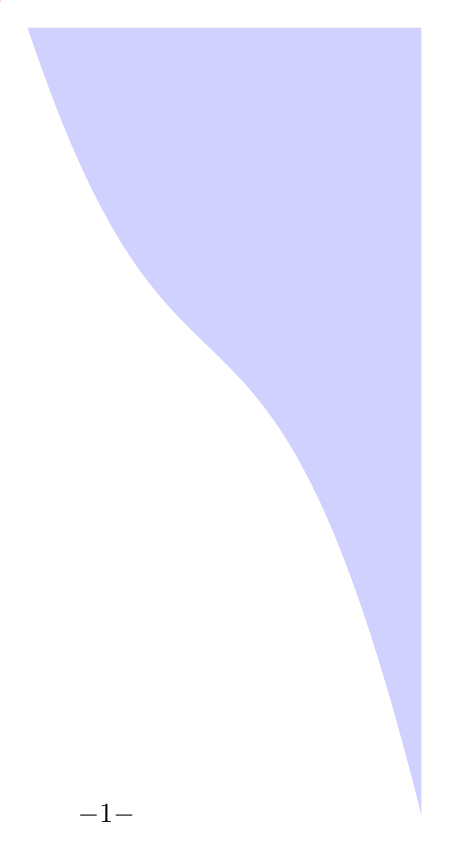
\begin{tikzpicture}
	\fill [blue!18](-5, 0) -- (0, 0) -- (0, -10) ..controls (-2, -2) and (-3, -6) ..(-5,0);
	\node at (-4, -10) {$- \thepage -$};
\end{tikzpicture}
}}

\maketitle

\newpage

{Copyright Simone Mosciatti 2016, Milano, Italy.}

This little booklet is intended as a short, and definitely not complete nor exhaustive, introduction to the problem and possible solution faced during the design of distributed, highly scalable, fault tolerant systems.

Following the Open Source principles this work is released under the Creative Commons, contributions and suggestions are extremely welcome. 

The complete source of the project can be found at \\
{\ttfamily https://github.com/siscia/intro-to-distributed-system} \\
where contributions are encouraged.

The author can be directly contacted through Twitter {\ttfamily @siscia\_} or via email at {\ttfamily simone@mweb.biz}

\vspace{\fill}

\begin{figure}[h]
	\centering
	\includegraphics{by-sa}
\end{figure}

{\small This work is licensed under the Creative Commons Attribution-ShareAlike 4.0 International License. To view a copy of this license, visit {\ttfamily http://creativecommons.org/licenses/by-sa/4.0/} .}

\section{Introduction}

In the last few years, the web has been exponentially growing and it is expected to keep growing faster than ever, accordingly the computing power required and the networking necessities need to be improved.

However our computers are not getting much faster, they have reached their physically limit regarding performance, but fortunately those machines are getting cheaper and more power efficient every single day.

The next logical step is thus to use a lot of cheap, small and power efficient computers instead of a few, big, expensive ones.

Computation is going to be divided between a lot of machines, likely, not even in the same datacenter. This will allow to build systems that have the necessary performance for the modern web but it will also bring its own set of problems and challenges.

Build and use distributed system is known to be very hard, but why?

\section{Why is it hard?}

Distributed systems are based on completely different foundations from traditional systems. The difference is that in the distributed systems there is not a physical central point of control where all the data flow; moreover information travel between the different parts of the system in a not negligible time.

Also there is expectation that our system is live 24/7/365. Using a single machine there is no way to defend ourselves against power loss or somebody tripping on the cables, but if we use a lot of small machines distributed in different parts of the globe there is no reason that our system should be down if problems occur in a single data center. 

Working in a distributed system means using more than a single machine. It is good because it means that your system could be resistant to failure, however having a lot of machines around it means that some of those will break no matter what.

Suppose that a machine goes ``down'' (whatever that means) with a small probability, lets say 1\%. This mean that a machine is ``up'' with a probability of $ 100\%-1\% = 99\%$. Now suppose you have 100 machines, it means that the probability that all machines are up at the same time is roughly $ 0.99^{100} = 0.366 $. What happens with 1000 machines? $0.99 ^ {1000} = 0,000043171 \approx 0 \%$ of chances of having all your computers ``up''.

In a big distributed system, at any given time, some machines will be ``down'' , some other machines will be having some weird problems and -- even worse -- some that were working just fine a couple of seconds ago will go down.

To manage all this complexity and uncertainty in a distributed system it is necessary to use a different mental framework from that used to build traditional systems.

	\subsection{State is evil}
	
As previously discussed, no matter what, some of your machines will go ``down'', they will completely lose their memory and you will have lost the state stored in those machines.

If your system relies on some state stored in a single machine you have a single point of failure, and when -- not if -- that machine goes down your system will go in some inconsistent state.

The simplest solution is to not keeping any state in your system, but this is not always a practicable solution. Keeping the number of state at the bare minimum is, likely, the best trade off possible.

When you lose state you need to be sure that your system can keep operating, it can either recover the state somehow (read it back from a persistent disk, ask to other part of the system or compute it back again from some known previous state) or, if the state wasn't so important, just don't care and keep going, which is arguably a wonderful solution as long as the system is operating correctly.

	\subsection{Forget about time}
	
Different machines have different clocks, they can be synchronized but it won't last.

Different clocks tick at different frequencies, the time on one machine is simply not reliable especially if events is necessary to be ordered.

It is also important to remember that if the machines are far away from each other there is a not negligible lag between the time when you send a message from San Francisco and the time when you receive that same message in London. 

	\subsection{Order of Events}
	
If it is not possible to rely on time, ordering events becomes harder. The only reliable way to order events is to make all the events pass through the same machine (ideally the same processor), however this doesn't scale very well.

If it is necessary to order a series of events, a good way is to keep a monotonic counter that can only increase and ask for a new value every time it is needed. Doing so, however, means keeping a state, and a very important one that is not possible to lose.

	\subsection{It is not that bad}

I have been very catastrophic, but it is never that bad. Most systems have strict requirements about something and more relaxed constraints about something else. 

In the chat system of a video game it is not such a big deal if one message gets lost. It would be nice if all messages would go through, but if one message in a million gets lost, nobody will complain, however such system may need to be up 24/7 and even a couple of minutes of downtime can mean a lot of lost profit.

On the other side a bank cannot afford to lose any transaction. If a payment needs a second attempt to go through it is annoying but still better than lose the customer's money.

It is important to understand what part of the system can be little more relaxed and where it is necessary to be extremely robust. A technological system, even if carefully designed, will always be limited, it is the designer's responsibility to make the system achieve the necessary performance.

\section{Small independent processes}

One way to build highly scalable, distributed systems is to use a lot of small independent units.

These units need to be stoppable and resumable at will.

Each unit will have some responsibility and will be able to keep some sort of state.

Since we are going to need a lot of those units, creating a new one must be a very light and quick operation and it cannot use much memory, an operating system fork is out of the plate.

Fortunately a lot of programming languages provide something similar. These units are called process in Erlang/Elixir, tasklets or greenlets in python, Fiber in Java using Quasar or Actor using Akka, goroutines in golang and more.

I am going to refer to them as ``process'' from now onward.

The context switch between different processes is extremely low, almost negligible and it is not problematic. Similarly a process without state needs very few bytes of memory.

This means that a single processor can handle an awful lot of different processes while it can manage -- with reasonable performance -- only a handful of different threads.

	\subsection{Filling a jar with stone or sand?}
	
Suppose that your processor is a jar of glass, you want to use as much as possible of it, would you fill it with weird big rocks, threads, or with fine sand, processes?

It is clear that sand won't leave much empty space, while the rocks will leave a lot of air, unused resource, in the jar.

If you have a lot of processes and most of them are able to do meaningful work, your CPU will be totally used, yielding good performance.
	
	\subsection{Performance Bounds}

There are three main factors that can limit the performance of a system: CPU, RAM \& I/O.

A system bounded only by one of these is more desirable because easier to scale, either vertically or horizontally.

If a system is bounded only by its CPU the easiest way to manage bigger loads is to use a faster processor, if the system is bounded only by its memory, buying more RAM is the best solution and if a system is bounded only by the I/O a faster disk, SSD or better network can be used.

Similarly it is possible to scale horizontally, distribute the computation between more machines to have better use of your CPU or RAM, use a load balancer to accommodate requests if the network is saturating, etc...

But if a system at its performance peek uses the 70\% of the CPU, the I/O is pretty much free and the RAM is around the 65\%, there is not a clear path to sustain bigger loads.

Using small processes with just a little bit of attention will make bottlenecks clearer and simpler to spot.

	\subsection{Isolation and message passing}
	
All the advantages of using small processes go bust if they share memory.

If the memory is shared between processes there will be the need for coordination to mutate the variables. Coordination will slow down the execution, hence it is preferable to let every process have it own independent memory.

Processes cannot share memory, but they usually communicate via messages.

A message is sent from a process to another and left on the receiver mail box, the receiver will be in charge of looking at its own mail box and take action if necessary.

Keep in mind that if you need to send some data from a process to another, the data will be copied, a reference to a common shared value will not be used.

\section{Keep minimum overhead}

Now that we have understood the advantages that small isolated processes bring, let's look at some basic rules on how to use them and the most common mistakes.

There is a very simple golden path to follow when building complex systems.

\begin{enumerate}
	\item Make it work
	\item Make it right
	\item Make it fast
\end{enumerate}

In order to achieve the great performances required by the modern web, keep testing a system during every iteration is needed, don't have any assumptions about performance and correctness.

Said so a couple of suggestions:

	\subsection{Avoid single process bottlenecks}
	
One of the simplest way to make a system speedup is to get rid of your bottlenecks. If all the processes in the system need to communicate with a single process, in order to coordinate, or to look at some global value, that single process is, or is about to be, a bottleneck.

The system is to be designed avoiding such bottlenecks as much as possible.	

	\subsection{Keep it as simple as possible}

A lot of languages provide some sort of framework to build applications, in Erlang it would be OTP. They are very helpful to build any meaningful application but they come with some overhead that is not always necessary.

Both the framework used and the language primitives need to be very well understood so that one can always choose the smallest sufficient element to get the job done.

	\subsection{Don't couple elements together}

Ideally processes should have a simple and pure API. It means that it should do only one thing and that its output depends only on its input, not on some hidden state.

This is not always achievable, but the more ``pure processes'' you have the easier will be to reason about your system and the more flexible it will be.

\end{document}
